\documentclass[11pt,a4paper]{article}

\usepackage[margin=2.4cm]{geometry}
\usepackage{fontspec}
\usepackage{xeCJK}
\usepackage{graphicx}
\usepackage{booktabs}
\usepackage{array}
\usepackage{hyperref}
\usepackage{xcolor}
\usepackage{caption}

\setmainfont{FreeSerif}
\setsansfont{FreeSans}
\setmonofont{DejaVu Sans Mono}
\setCJKmainfont{Noto Serif CJK SC}
\setCJKsansfont{Noto Sans CJK SC}
\setCJKmonofont{Noto Sans Mono CJK SC}

\hypersetup{
  colorlinks=true,
  linkcolor=blue!55!black,
  urlcolor=blue!55!black,
  citecolor=blue!55!black
}

\title{Latent Diffusion Models 核心结论复现报告}
\author{复现实验：\texttt{latent-diffusion-cvpr2022-reproduction}}
\date{2026年4月17日}

\begin{document}
\maketitle

\section{复现目标}

Rombach 等人在 CVPR 2022 论文 \emph{High-Resolution Image Synthesis with Latent Diffusion Models} 中提出：先用感知自编码器把图像压缩到低维 latent 空间，再在 latent 空间训练扩散模型，可以在保留视觉质量的同时显著降低扩散模型的训练和采样成本。本文不从零训练大规模扩散模型，而是围绕论文的两个核心机制做可复现实验：第一，验证 first-stage autoencoder 的压缩--重建权衡；第二，使用官方预训练 LDM 复现 DDIM 采样步数与推理速度、样本质量之间的权衡。

具体实验包括：
\begin{itemize}
  \item 使用官方预训练 KL autoencoder，比较 \texttt{kl-f4}、\texttt{kl-f8}、\texttt{kl-f16} 三个下采样因子模型的重建质量、latent 表示大小和推理吞吐量。
  \item 使用官方 CelebA-HQ 256 无条件 LDM checkpoint，比较 DDIM steps 为 10、20、50、100、200 时的采样速度和生成样本。
\end{itemize}

\section{实验设置}

源码来自官方仓库 \url{https://github.com/CompVis/latent-diffusion}，放置于项目的 \texttt{src} 目录。复现实验代码位于项目的 \texttt{reproduction} 目录，报告和图片分别位于 \texttt{reports} 与 \texttt{reports/FIG}。

使用的官方 checkpoint 为：
\begin{itemize}
  \item \texttt{models/first\_stage\_models/kl-f4/model.ckpt}
  \item \texttt{models/first\_stage\_models/kl-f8/model.ckpt}
  \item \texttt{models/first\_stage\_models/kl-f16/model.ckpt}
  \item \texttt{models/ldm/celeba256/model.ckpt}
\end{itemize}

本次快速复现使用官方源码 \texttt{src/assets} 中的 12 张示例图像，统一 resize 并 center crop 到 $256\times256$。输入像素值映射到 $[-1,1]$ 后输入 autoencoder，重建结果再映射回 $[0,1]$。实验环境为 \texttt{DDCSR} conda 环境，PyTorch 2.4.1，CUDA 12.1，GPU 为 NVIDIA H100 PCIe。复现实验命令为：

\begin{verbatim}
conda run -n DDCSR python reproduction/run_autoencoder_tradeoff.py \
  --device cuda:1 --batch-size 4 --num-images 12
\end{verbatim}

LDM 采样实验使用官方 CelebA-HQ 256 无条件模型，采样时切换到 checkpoint 中的 EMA 权重。实验固定 batch size 为 4、DDIM $\eta=0$、随机种子为 20260417，并丢弃一次 5-step warmup 后再计时。由于官方 DDIM sampler 默认使用 \texttt{cuda} 设备，本次运行通过 \texttt{CUDA\_VISIBLE\_DEVICES=1} 指向空闲 H100：

\begin{verbatim}
CUDA_VISIBLE_DEVICES=1 conda run -n DDCSR \
  python reproduction/run_ldm_sampling_benchmark.py \
  --steps 10 20 50 100 200 --batch-size 4 --eta 0.0 --device cuda
\end{verbatim}

autoencoder 实验指标包括 MSE、PSNR、一个轻量全局 SSIM 指标、latent 表示元素数量、latent/像素表示比例和端到端 images/s。论文对照值取自官方 README 中 first-stage KL autoencoder 表格，即论文 Table 8 对应模型库结果。需要强调的是，本文指标和论文指标不是同一测试协议下的逐项复算：本文使用 12 张官方示例图做快速验证，论文结果来自大规模验证集和官方评价流程。因此下表用于比较趋势，而不是声称本文 PSNR 应当与论文 PSNR 完全一致。

\section{数值结果}

\begin{table}[htbp]
\centering
\small
\caption{KL autoencoder 压缩率与重建质量对照。左侧为本文在 12 张官方示例图上的快速复现结果，右侧为论文/官方模型库给出的参考结果；两者数据集和评价协议不同，因此主要比较随 $f$ 变化的趋势。}
\begin{tabular}{lccccc cc}
\toprule
 & & & \multicolumn{3}{c}{本文：12 张官方示例图} & \multicolumn{2}{c}{论文/官方参考} \\
\cmidrule(lr){4-6}\cmidrule(lr){7-8}
模型 & 压缩因子 $f$ & latent 形状 & latent/像素 & PSNR$\uparrow$ & SSIM$\uparrow$ & PSNR$\uparrow$ & rFID$\downarrow$ \\
\midrule
\texttt{kl-f4}  & 4  & $3\times64\times64$   & 6.25\% & 32.07 & 0.995 & 27.53 & 0.27 \\
\texttt{kl-f8}  & 8  & $4\times32\times32$   & 2.08\% & 28.33 & 0.985 & 24.19 & 0.90 \\
\texttt{kl-f16} & 16 & $16\times16\times16$  & 2.08\% & 27.48 & 0.982 & 24.08 & 0.87 \\
\bottomrule
\end{tabular}
\end{table}

本次实验中，\texttt{kl-f4} 的 PSNR 为 32.07 dB，明显高于 \texttt{kl-f8} 的 28.33 dB 和 \texttt{kl-f16} 的 27.48 dB。latent 表示大小从原图 $3\times256\times256=196608$ 个数值降到 \texttt{kl-f4} 的 12288 个数值，仅为原来的 6.25\%；\texttt{kl-f8} 和 \texttt{kl-f16} 均为 4096 个数值，仅为原来的 2.08\%。这验证了论文的核心机制：first-stage autoencoder 能在很小的 latent 空间中保留图像主体内容，从而使后续扩散模型不必直接在像素空间建模。

本文 PSNR 普遍高于论文表格中的 PSNR，主要有三点原因。第一，本文只使用 12 张官方示例图，样本少且图像相对规整；论文结果来自大规模验证集，图像内容分布更复杂。第二，本文使用固定的 resize 与 center crop，并用 posterior mode 做确定性重建；论文评价流程、数据 split 和预处理并不与本文完全相同。第三，rFID 是基于大量真实图像和重建图像的 Inception 特征分布距离，12 张图无法稳定估计，因此本文没有重新报告 rFID，而只引用论文/官方参考值。由此，合理的比较方式是看趋势：在两套结果中，较小的压缩因子通常对应更好的重建质量，而更大的压缩带来更低的 latent 表示成本。

\begin{figure}[htbp]
\centering
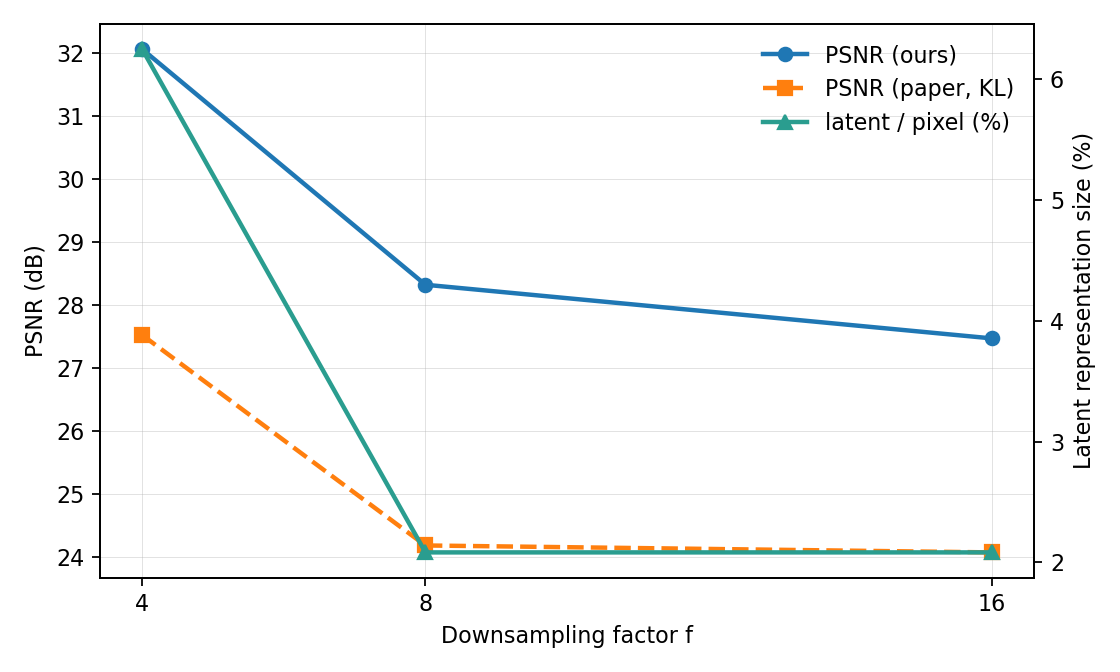
\includegraphics[width=\linewidth]{FIG/metrics_tradeoff.png}
\caption{PSNR 与 latent 表示比例的权衡。随着 $f$ 增大，latent 表示更小、推理更快，但重建质量下降。}
\end{figure}

\begin{figure}[htbp]
\centering
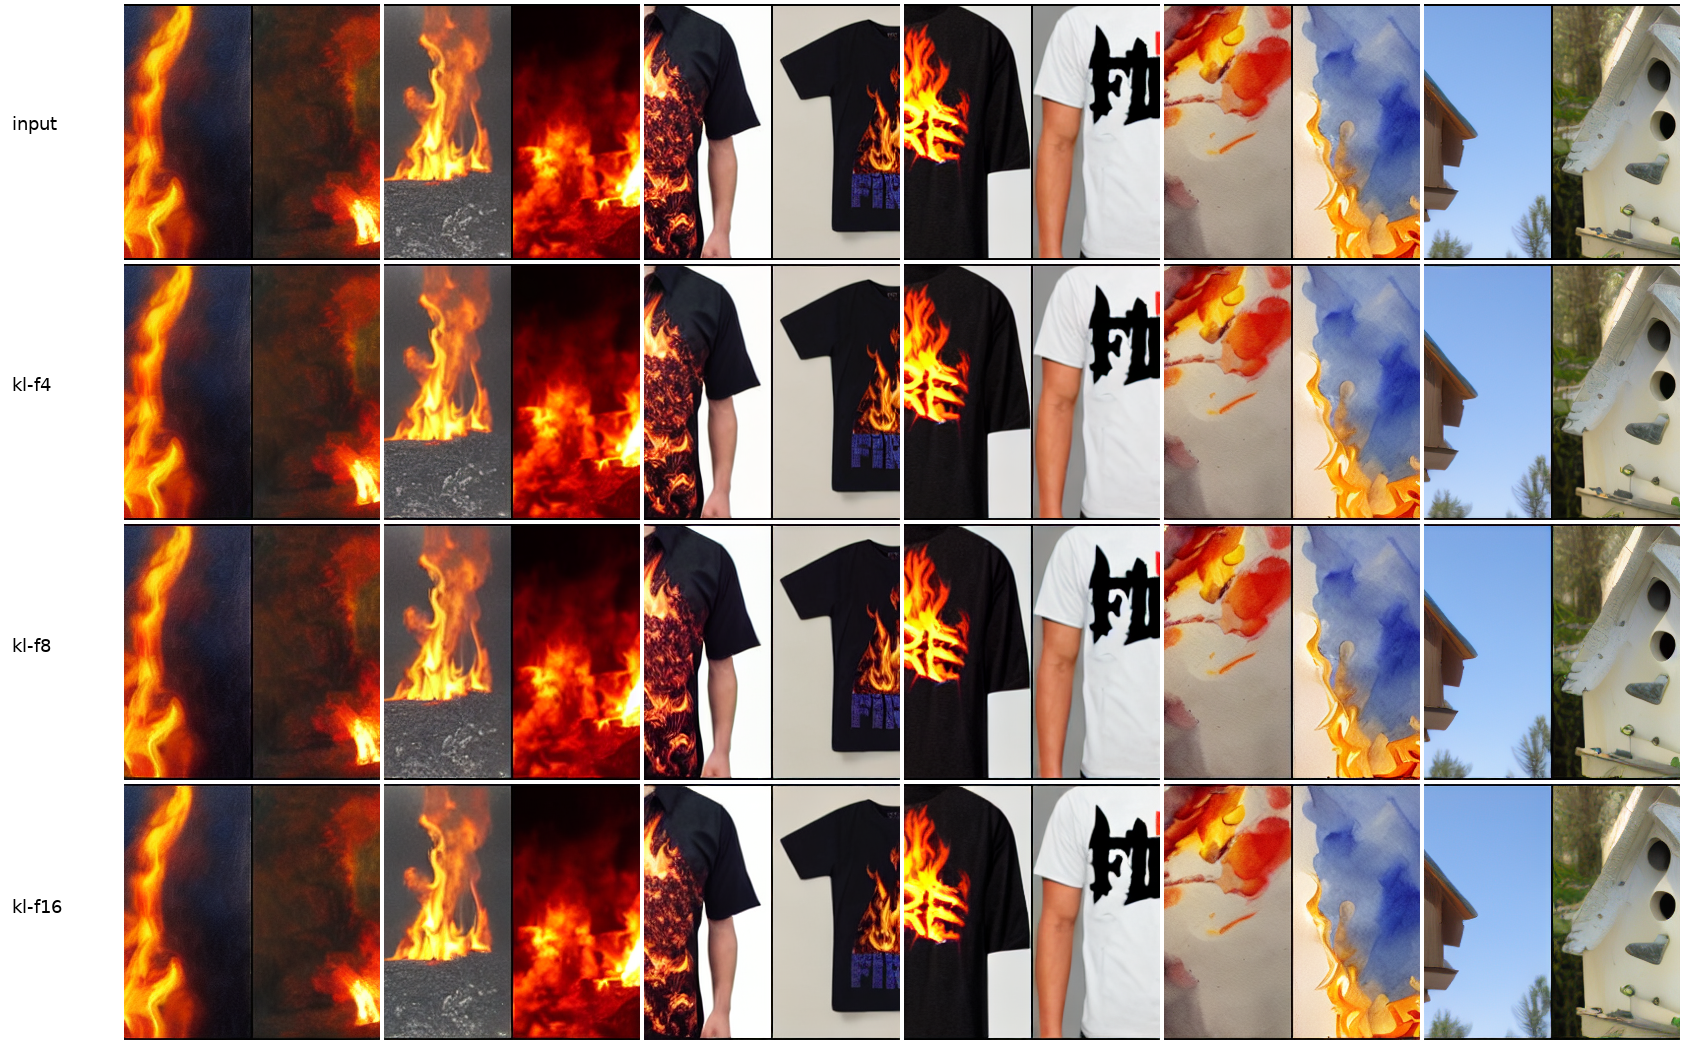
\includegraphics[width=\linewidth]{FIG/reconstruction_grid.png}
\caption{输入图像与三个 KL autoencoder 的重建结果。$f=4$ 细节保留最好；更强压缩会带来纹理和边缘细节损失。}
\end{figure}

\begin{table}[htbp]
\centering
\small
\caption{官方 CelebA-HQ 256 LDM 的 DDIM 采样运行时。每组生成 4 张图，计时包含 latent denoising 和 first-stage decode，并已丢弃一次 warmup。}
\begin{tabular}{rrrrr}
\toprule
DDIM steps & 总时间(s) & 单图时间(s/img) & 吞吐量(img/s) & decode 时间(s) \\
\midrule
10  & 0.282 & 0.071 & 14.17 & 0.041 \\
20  & 0.474 & 0.119 &  8.44 & 0.041 \\
50  & 1.122 & 0.280 &  3.57 & 0.041 \\
100 & 2.274 & 0.568 &  1.76 & 0.041 \\
200 & 4.389 & 1.097 &  0.91 & 0.041 \\
\bottomrule
\end{tabular}
\end{table}

\begin{figure}[htbp]
\centering
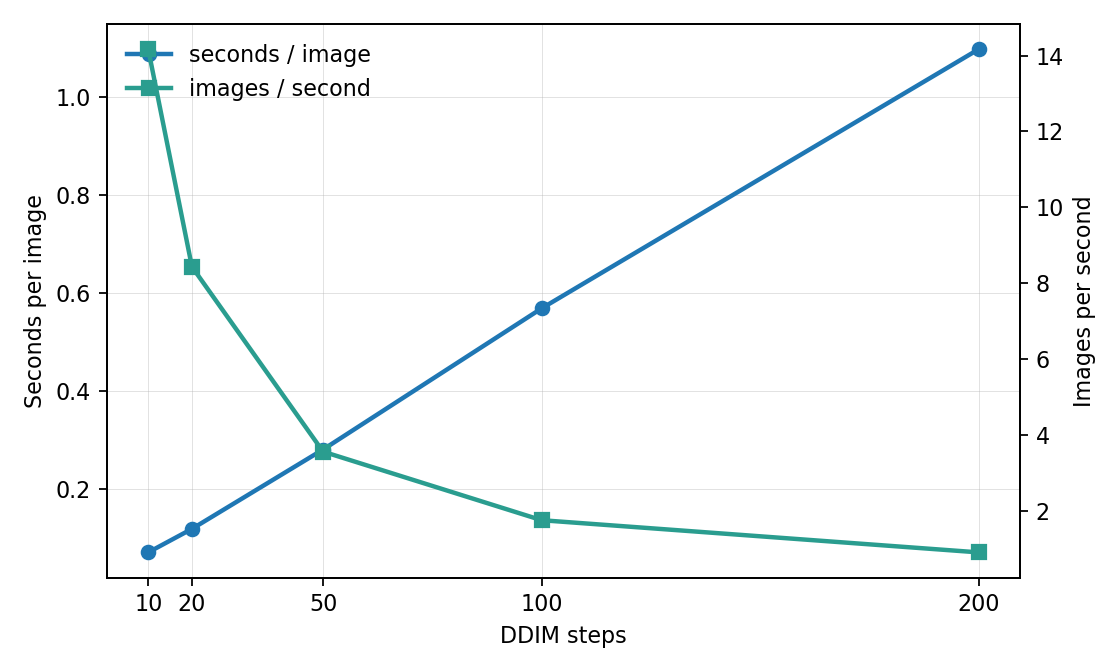
\includegraphics[width=\linewidth]{FIG/ddim_sampling_runtime.png}
\caption{DDIM steps 与采样速度的关系。步数增加时，单图时间近似线性上升，吞吐量下降。}
\end{figure}

\begin{figure}[htbp]
\centering
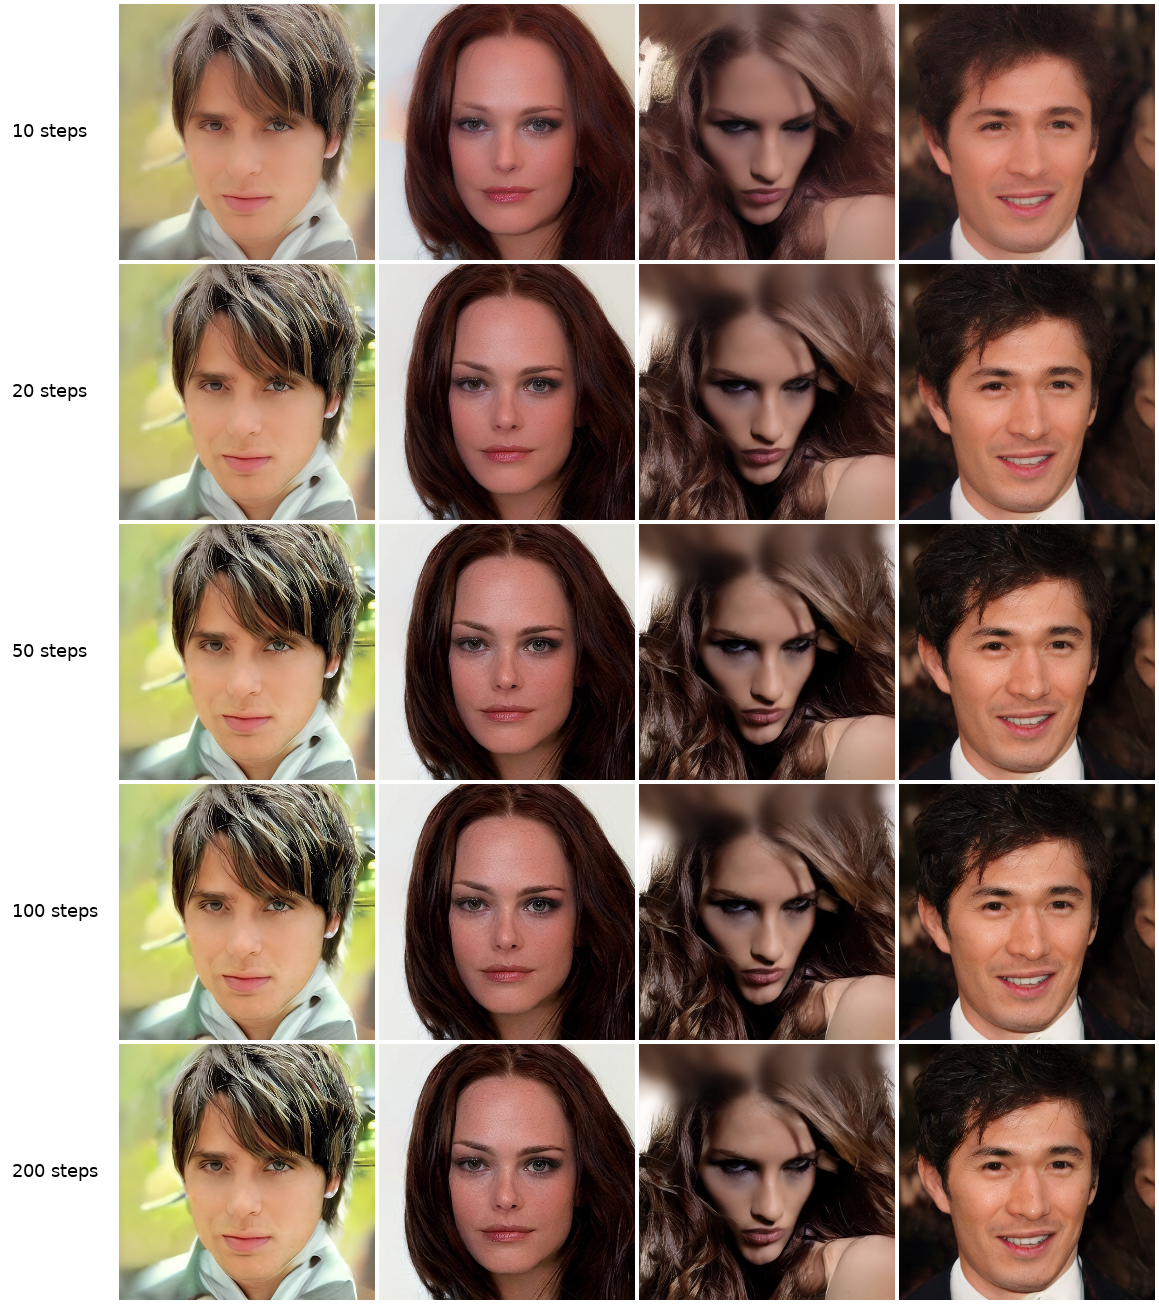
\includegraphics[width=0.92\linewidth]{FIG/ddim_steps_samples.png}
\caption{同一初始噪声下不同 DDIM steps 的 CelebA-HQ LDM 生成结果。少步数采样速度快，但局部结构和纹理更不稳定；更多步数带来更充分的去噪过程。}
\end{figure}

\section{与论文结论的比较}

论文的结论不是简单追求最小 latent，而是在重建质量、语义保真和扩散模型计算成本之间寻找折中。本文复现实验支持这一点：

\begin{itemize}
  \item \textbf{适度压缩保留质量。} \texttt{kl-f4} 的 latent 仅为像素表示的 6.25\%，但在本文样本上仍达到 32.07 dB PSNR 和 0.995 SSIM；论文模型库中 \texttt{kl-f4} 也给出最高的 KL 组 PSNR 27.53 和最低 rFID 0.27。
  \item \textbf{过强压缩降低重建细节。} 从 \texttt{kl-f4} 到 \texttt{kl-f8}/\texttt{kl-f16}，本文 PSNR 分别下降约 3.74 dB 和 4.59 dB，视觉上边缘和局部纹理更容易变平滑。
  \item \textbf{latent 空间带来计算收益。} 在本机 H100 上，吞吐量从 \texttt{kl-f4} 的 14.58 images/s 提升到 \texttt{kl-f8} 的 65.95 images/s、\texttt{kl-f16} 的 90.26 images/s。尽管该吞吐量只测 autoencoder 前向过程，不等同于完整 LDM 采样速度，但它反映了更小 latent 空间的计算优势。
  \item \textbf{DDIM 步数形成速度--质量权衡。} CelebA-HQ LDM 采样中，10 steps 的单图时间为 0.071 s，而 200 steps 增加到 1.097 s。该趋势对应论文 Fig. 6 的基本观察：增加 denoising steps 通常改善采样过程，但会按步数增加计算成本。
\end{itemize}

\section{结论}

本次复现使用官方代码、官方 KL autoencoder checkpoint 和官方 CelebA-HQ LDM checkpoint，得到与论文一致的两个核心趋势：\texttt{f=4} 的 mild compression 在保真度上最好，同时已把表示规模压缩到像素空间的 6.25\%；DDIM 采样步数越多，生成过程耗时越高。二者共同支持论文选择在 latent 空间训练扩散模型的核心理由，即把扩散模型从高维像素空间迁移到感知等价但计算更低的 latent 空间，并通过可调采样步数在速度和质量之间折中。

\end{document}
